% !TEX TS-program = XeLaTeX
% Commands for running this example:
% 	 xelatex parabola-plot
% End of Commands
\documentclass{article}
\pagestyle{empty}
\usepackage{tikz,amssymb,amsmath,tikz-cd}
\usetikzlibrary{patterns}\usepackage[left=1.5cm,right=1.5cm]{geometry}
\usepackage{xepersian}

\newcommand{\mes}[1]{
\begin{center}
 \tikzstyle{mybox} = [draw=red, fill=gray!0, very thick,
    rectangle, rounded corners, inner sep=10pt, inner ysep=20pt]
\tikzstyle{fancytitle} =[fill=red, text=white]
\begin{tikzpicture}
\node [mybox] (box)\ \ \ 
};
\node[fancytitle, rounded corners] at (box.north) {\hboxR{خروجی}};
\end{tikzpicture}%
\end{center}
}
\def\ba{\backslash}
\begin{document}
فرم کلی مختصات به صورت دکارتی $(x,y)$ یا قطبی $(\theta: r)$  (به مرکزیت مبدا مختصات می‌باشد).\\

رسم خطوط :

  مختصات نقاطی که خط از آنها عبور می‌کند  به شکل زیر داده می‌شود.
\begin{latin}\begin{verbatim}
\draw[option] (x_0,y_0) -- (x_1,y_1) ... --(x_n,y_n);
\end{verbatim}\end{latin}
پارامتر‌های 
\lr{line width=dim}
 و 
 \lr{draw=color}
  برای تغییر ضخامت و رنگ خط بکار می‌رود. در خطوط شکسته می‌توان با استفاده از پارامتر
 \lr{rounded corners=dim}
 گوشه‌های تیز را از بین برد. برا جهت دار کردن خط از علائم $<$ و $>$ استفاده می‌کنیم. از آپشن‌های زیر نیز  برای تغییر حالت خط به فرم‌هایی چون 
 نقطه‌چین، خط‌چین، $\ldots$   استفاده می‌شود.
 
 \begin{latin}
\begin{tabular}{||l|l|l|l||}\hline
 solid&  dotted& densely dotted& loosely dotted\\\hline
 dashed& densely dashed&  loosely dashed& dashdotted\\\hline
 densely dashdotted& loosely dashdotted& dashdotdotted& densely dashdotdotted\\\hline
  loosely dashdotdotted&&&\\\hline
\end{tabular}\end{latin} 
نام برخی از رنگهای پیش فرض عبارتند از:
\begin{latin}
\begin{tabular}{|c|c|c|c|c|c|c|c|}
\hline
red  & green  & blue &cyan  &magenta  &yellow  &black  &gray  \\ 
\hline 
\tikz \draw [red, line width=6]
(0,0) -- (.5,0); &
\tikz \draw [green, line width=6]
(0,0) -- (.5,0);  &
\tikz \draw [blue, line width=6]
(0,0) -- (.5,0);  & 
\tikz \draw [cyan, line width=6]
(0,0) -- (.5,0); &
\tikz \draw [magenta, line width=6]
(0,0) -- (.5,0);  &
\tikz \draw [yellow, line width=6]
(0,0) -- (.5,0);  &  
\tikz \draw [black, line width=6]
(0,0) -- (.5,0);& 
\tikz \draw [gray, line width=6]
(0,0) -- (.5,0); \\ 
\hline 
darkgray  & lightgray & brown &lime  &olive  &orange  &pink  &purpla  \\ 
\hline 
\tikz \draw [darkgray, line width=6]
(0,0) -- (.5,0); &
\tikz \draw [lightgray, line width=6]
(0,0) -- (.5,0);  &
\tikz \draw [brown, line width=6]
(0,0) -- (.5,0);  & 
\tikz \draw [lime, line width=6]
(0,0) -- (.5,0); &
\tikz \draw [olive, line width=6]
(0,0) -- (.5,0);  &
\tikz \draw [orange, line width=6]
(0,0) -- (.5,0);  &  
\tikz \draw [pink, line width=6]
(0,0) -- (.5,0);& 
\tikz \draw [purple, line width=6]
(0,0) -- (.5,0); \\ \hline
teal  & violet & white &  &  &  &  &  \\ 
\hline 
\tikz \draw [teal, line width=6]
(0,0) -- (.5,0); &
\tikz \draw [violet, line width=6]
(0,0) -- (.5,0);  &
\tikz \draw [fill=white]
(0,0) rectangle (.5,.2);  & 
 &  &  &  & 
 \\ \hline
\end{tabular} 
\end{latin}

مثال:



%____________________________________________
 \begin{latin}
 \tikzstyle{mybox} = [draw=red, fill=gray!0, very thick,
    rectangle, inner sep=10pt, inner ysep=20pt]
\tikzstyle{fancytitle} =[fill=red, text=black]
\begin{tikzpicture}
\node [mybox] (box){%
  \begin{minipage}{0.42\textwidth}
 \begin{verbatim}
\begin{tikzpicture}
\draw (0,0) -- (1,2);
\draw  [line width=5pt,draw=red]
(1.2,0) -- (2,1) -- (3,.5);
\draw[->,rounded
 corners=6pt,line width=2pt,blue]%
 (0,4) -- (1,3) -- (1.5,3.7) -- (2,3);
\draw[line width=2pt,dashed] 
(4,2) -- (5,3) -- (6,2.5) -- (4,2);
\draw (6,0) -- (30:3);
\end{tikzpicture}
\end{verbatim}

\end{minipage}%\tikzstyle{ali}=[]
\fboxrule=1mm\fbox{    \begin{minipage}{0.42\textwidth}
%%%%%%%%%%%%%%%%%%%%%%%%%%%%%%%%%%
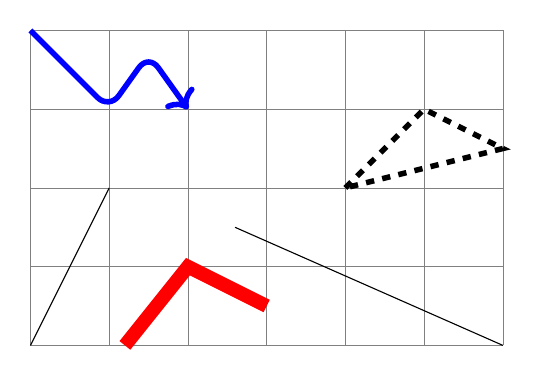
\begin{tikzpicture}
\draw[help lines,step=1cm] (0,0) grid (6,4);
\draw (0,0) -- (1,2);
\draw  [line width=5pt,draw=red](1.2,0) -- (2,1) -- (3,.5);
\draw[->,rounded corners=6pt,line width=2pt,blue]%
 (0,4) -- (1,3) -- (1.5,3.7) -- (2,3);
\draw[line width=2pt,dashed] (4,2) -- (5,3) -- (6,2.5) -- (4,2);
\draw (6,0) -- (30:3);
\end{tikzpicture}
%%%%%%%%%%%%%%%%%%%%%%%%%%%%%%%%% 
    \end{minipage}}
    } ;
\node[above=0pt,fancytitle,right=10pt] at (box.north) {\hboxL{Output}};
\node[above=0pt,fancytitle, left=-50pt] at (box.north west) {\hboxL{Input}};

\end{tikzpicture}%
\end{latin}
%____________________________________________


برای رسم خط  می‌توان مقادیری که به  $x$ , $y$ نسبت به نقطه اولیه اضافه می‌شوند را به صورت 
$++(\bigtriangleup x, \bigtriangleup y)$
 وارد نمود.\\
  مثال \\
  %____________________________________________
 \begin{latin}
 \tikzstyle{mybox} = [draw=red, fill=gray!0, very thick,
    rectangle, inner sep=10pt, inner ysep=20pt]
\tikzstyle{fancytitle} =[fill=red, text=black]
\begin{tikzpicture}
\node [mybox] (box){%
  \begin{minipage}{0.42\textwidth}
 \begin{verbatim}
\begin{tikzpicture}
\draw[step=1cm,gray,very thin]
 (-.4,-.4) grid (4.4,2.4);
\draw (0,0) -- ++(2,1) -- ++(2,0);
\end{tikzpicture}
\end{verbatim}

    \end{minipage}
\fboxrule=1mm\fbox{  \begin{minipage}{0.42\textwidth}
%%%%%%%%%%%%%%%%%%%%%%%%%%%%%%%%%%
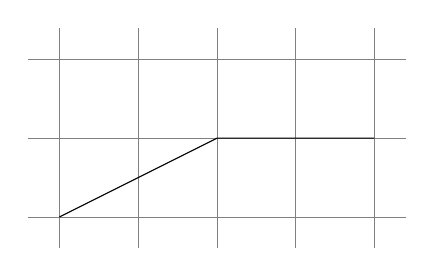
\begin{tikzpicture}
\draw[step=1cm,gray,very thin] (-.4,-.4) grid (4.4,2.4);
\draw (0,0) -- ++(2,1) -- ++(2,0);
\end{tikzpicture}
%%%%%%%%%%%%%%%%%%%%%%%%%%%%%%%%% 
    \end{minipage}}
    } ;
\node[fancytitle, right=10pt] at (box.north) {\hboxL{Output}};
\node[fancytitle, left=-50pt] at (box.north west) {\hboxL{Input}};

\end{tikzpicture}%
\end{latin}
%____________________________________________

 در مثال بالا مولفه اول  نقطه دوم با اضافه کردن ۲ واحد به صفر و مولفه دوم آن با ضافه کردن ۱ واحد به صفر بدست می‌آید. همچنین برای مولفه اول نقطه
سوم ۲ واحد به نقطه دوم اضافه می‌کنیم. در واقع در این روش هر نقطه جدید  از نقطه قبل از خود بدست می‌آید. چنانچه
 بجای دو علامت + از یک علامت استفاده کنیم ، تمام نقاطی که به این روش بدست می‌آیند نسبت به نقطه اولیه محاسبه می‌شوند.\\
 مثال \\
  %____________________________________________
 \begin{latin} \tikzstyle{mybox} = [draw=red, fill=gray!0, very thick,rectangle, inner sep=10pt, inner ysep=20pt]
\tikzstyle{fancytitle} =[fill=red, text=black]\begin{tikzpicture}
\node [mybox] (box){\begin{minipage}{0.42\textwidth}\begin{verbatim}
 %******************************
\begin{tikzpicture}
\draw[step=1cm,gray,very thin] 
(-.4,-.4) grid (4.4,2.4);
\draw (0,0) -- +(2,1) -- +(2,0);
\end{tikzpicture}
%*******************************
\end{verbatim}
    \end{minipage}
\fboxrule=1mm\fbox{  \begin{minipage}{0.42\textwidth}
%%%%%%%%%%%%%%%%%%%%%%%%%%%%%%%%%%
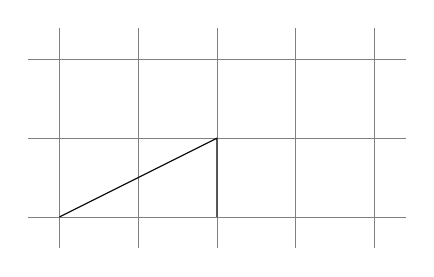
\begin{tikzpicture}
\draw[step=1cm,gray,very thin] (-.4,-.4) grid (4.4,2.4);
\draw (0,0) -- +(2,1) -- +(2,0);
\end{tikzpicture}
%%%%%%%%%%%%%%%%%%%%%%%%%%%%%%%%% 
    \end{minipage}}} ;\node[fancytitle, right=10pt] at (box.north) {\hboxL{Output}};\node[fancytitle, left=-50pt] at (box.north west) {\hboxL{Input}};
\end{tikzpicture}\end{latin}
%____________________________________________


 فراخوانی آپشن 
\lr{arrows}
به شکل 
\begin{latin}
\begin{verbatim}\usetikzlibrary{arrows}
\end{verbatim}
\end{latin}
 دستیابی به کنترل بیشتر روی  نوک پیکان‌ها را بهبود می‌بخشد.
  
  مثال \\
\usetikzlibrary{arrows}   %____________________________________________
 \begin{latin} \tikzstyle{mybox} = [draw=red, fill=gray!0, very thick,rectangle, inner sep=10pt, inner ysep=20pt]
\tikzstyle{fancytitle} =[fill=red, text=black]\begin{tikzpicture}
\node [mybox] (box){\begin{minipage}{0.42\textwidth}\begin{verbatim}
 %******************************
\begin{tikzpicture}
\draw[->,>=triangle 45] ( 1, 0) -- ( 0, 1);
\draw[->,>=triangle 45] ( 0, 1) -- (-1, 0);
\draw[->,>=triangle 60] (-1, 0) -- ( 0,-1);
\draw[->,>=triangle 90] ( 0,-1) -- ( 1, 0);
\end{tikzpicture}
%*******************************
\end{verbatim}
    \end{minipage}
\fboxrule=1mm\fbox{  \begin{minipage}{0.42\textwidth}
%%%%%%%%%%%%%%%%%%%%%%%%%%%%%%%%%%
\usetikzlibrary{arrows}
\begin{tikzpicture}
\draw[>=open triangle 45, <->] ( 1, 0) -- ( 0, 1);
\draw[>=latex, <-|] ( 0, 1) -- (-1, 0);
\draw[->,>=triangle 60] (-1, 0) -- ( 0,-1);
\draw[->,>=triangle 90] ( 0,-1) -- ( 1, 0);
\end{tikzpicture}
%%%%%%%%%%%%%%%%%%%%%%%%%%%%%%%%% 
    \end{minipage}}} ;\node[fancytitle, right=10pt] at (box.north) {\hboxL{Output}};\node[fancytitle, left=-50pt] at (box.north west) {\hboxL{Input}};
\end{tikzpicture}\end{latin}
%____________________________________________


 در ترسیمات مختلف می‌توان مختصات نقطه را به صورت قطبی 
 $(\theta :r)$
 وارد نمود. همچنین محدودیتی در این کار وجود ندارد. یعنی می‌توان مختصات برخی نقاط را دکارتی و برخی دیگر را قطبی وارد نمایید. می‌توان مولفه‌ها را بصورت اعداد توان دارد یا مجموعی از اعداد وارد نمود
 \\
 مثال \\
 
 
   %____________________________________________
 \begin{latin} \tikzstyle{mybox} = [draw=red, fill=gray!0, very thick,rectangle, inner sep=10pt, inner ysep=20pt]
\tikzstyle{fancytitle} =[fill=red, text=black]\begin{tikzpicture}
\node [mybox] (box){\begin{minipage}{0.42\textwidth}
\begin{footnotesize}\begin{verbatim}
 %******************************
\begin{tikzpicture}
\draw[line width=2pt] (0,0) -- (0:1) --(30:1);
\draw[line width=2pt] (2,0) -- (2+1,2^.5);
\draw[line width=2pt] (2*2,0) -- (4,1);
\end{tikzpicture}
%*******************************
\end{verbatim}\end{footnotesize}
    \end{minipage}
\fboxrule=1mm\fbox{  \begin{minipage}{0.42\textwidth}
%%%%%%%%%%%%%%%%%%%%%%%%%%%%%%%%%%
\usetikzlibrary{arrows}
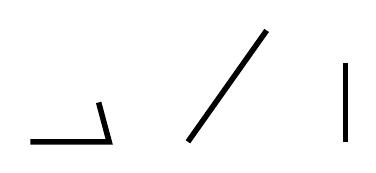
\begin{tikzpicture}
\draw[line width=2pt] (0,0) -- (0:1) --(30:1);
\draw[line width=2pt] (2,0) -- (2+1,2^.5);
\draw[line width=2pt] (2*2,0) -- (4,1);
\end{tikzpicture}
%%%%%%%%%%%%%%%%%%%%%%%%%%%%%%%%% 
    \end{minipage}}} ;\node[fancytitle, right=10pt] at (box.north) {\hboxL{Output}};\node[fancytitle, left=-50pt] at (box.north west) {\hboxL{Input}};
\end{tikzpicture}\end{latin}
%____________________________________________


می‌توان هنگام اتصال دو نقطه با استفاده  دستور $to$ و آپشن‌های 
\lr{out=deg}
 و 
 \lr{in=deg}
 زاویه خروج خط از نقطه شروه و ورود آن به نقطه پایانی، انحنای دلخواهی به خط اتصال داد.\\
 مثال \\
 
   %____________________________________________
 \begin{latin} \tikzstyle{mybox} = [draw=red, fill=gray!0, very thick,rectangle, inner sep=10pt, inner ysep=20pt]
\tikzstyle{fancytitle} =[fill=red, text=black]\begin{tikzpicture}
\node [mybox] (box){\begin{minipage}{0.42\textwidth}
\begin{footnotesize}\begin{verbatim}
 %******************************
\begin{tikzpicture}
\draw[very thick] (0,0) to [out=90,in=195] (2,0);
\draw[very thick] (2.5,0) to [out=90,in=90] (3.5,0);
\draw[very thick] (4.5,0) to [out=45,in=135] 
(5.5,0) to [out=-45,in=-135] (6,0) ;
\draw [<->,thick, cyan] (0,3) to [out=90,in=180] (1,4)
to [out=0,in=180] (2.5,3) to [out=0,in=-135] (4,4) ;
\end{tikzpicture}
%*******************************
\end{verbatim}\end{footnotesize}
    \end{minipage}
\fboxrule=1mm\fbox{  \begin{minipage}{0.42\textwidth}
%%%%%%%%%%%%%%%%%%%%%%%%%%%%%%%%%%
\begin{tikzpicture}
\draw[very thick] (0,0) to [out=90,in=195] (2,0);
\draw[very thick] (2.5,0) to [out=90,in=90] (3.5,0);
\draw[very thick] (4.5,0) to [out=45,in=135] (5.5,0) to [out=-45,in=-135] (6,0) ;
\draw [<->,thick, cyan] (0,3) to [out=90,in=180] (1,4)
to [out=0,in=180] (2.5,3) to [out=0,in=-135] (4,4) ;
\end{tikzpicture}
%%%%%%%%%%%%%%%%%%%%%%%%%%%%%%%%% 
    \end{minipage}}} ;\node[fancytitle, right=10pt] at (box.north) {\hboxL{Output}};\node[fancytitle, left=-50pt] at (box.north west) {\hboxL{Input}};
\end{tikzpicture}\end{latin}
%____________________________________________
 بدیهی است که در رسم خطوط اگر نقطه انتهایی و ابتدایی یکی باشد یک ناحیه بسته ترسیم می‌گرد. بطور کلی چنانچه بخاهیم از آخرین نقطه هر ترسیمی به نقطه ابتدای وصل گردد می‌توان بجای مختصات نقطه اولیه در انتها  دستور 
 \lr{cycle}
  را وارد نمود.
 
 مثال \\
   %____________________________________________
 \begin{latin} \tikzstyle{mybox} = [draw=red, fill=gray!0, very thick,rectangle, inner sep=10pt, inner ysep=20pt]
\tikzstyle{fancytitle} =[fill=red, text=black]\begin{tikzpicture}
\node [mybox] (box){\begin{minipage}{0.42\textwidth}
\begin{footnotesize}\begin{verbatim}
 %******************************
\begin{tikzpicture}
\draw[step=0.25cm,color=gray] (-1,-1) grid (1,1);
\draw (1,0) -- (0,1) -- (-1,0) -- (0,-1) -- cycle;
\end{tikzpicture}
%*******************************
\end{verbatim}\end{footnotesize}
    \end{minipage}
\fboxrule=1mm\fbox{  \begin{minipage}{0.42\textwidth}
%%%%%%%%%%%%%%%%%%%%%%%%%%%%%%%%%%
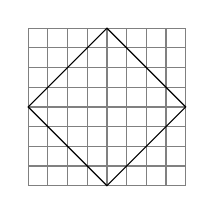
\begin{tikzpicture}
\draw[step=0.25cm,color=gray] (-1,-1) grid (1,1);
\draw (1,0) -- (0,1) -- (-1,0) -- (0,-1) -- cycle;
\end{tikzpicture}
%%%%%%%%%%%%%%%%%%%%%%%%%%%%%%%%% 
    \end{minipage}}} ;\node[fancytitle, right=10pt] at (box.north) {\hboxL{Output}};\node[fancytitle, left=-50pt] at (box.north west) {\hboxL{Input}};
\end{tikzpicture}\end{latin}
%____________________________________________
 

  
برای رسم مستطیل می‌توان   اضلاع آن را رسم نمود اما روش ساده‌تر آن است  مختصات دو گوشه مقابل به هم از مستطیل  به شکل زیر داده می‌شود. 

\begin{flushleft}
$\backslash draw  (x_0,y_0)\ rectangle\ (x_1,y_1);$
\end{flushleft}
 و یا با استفاده از علامت$+$ می‌توان مختصات یک گوشه را داد و به مقدار دلخواه به طول و عرض این نقطه اضافه نمود 
 
 مثال  \\
 
 
 %____________________________________________
 \begin{latin} \tikzstyle{mybox} = [draw=red, fill=gray!0, very thick,rectangle, inner sep=10pt, inner ysep=20pt]
\tikzstyle{fancytitle} =[fill=red, text=black]\begin{tikzpicture}
\node [mybox] (box){\begin{minipage}{0.42\textwidth}
\begin{footnotesize}\begin{verbatim}
 %******************************
\begin{tikzpicture}
\draw (0,0) rectangle (2,1);
\draw (-0.5,-0.5) rectangle (-1,-1);
\draw (3,0) rectangle +(1.5,1);
\draw (5,1) rectangle +(1,-1);
\end{tikzpicture}
%*******************************
\end{verbatim}\end{footnotesize}
    \end{minipage}
\fboxrule=1mm\fbox{  \begin{minipage}{0.42\textwidth}
%%%%%%%%%%%%%%%%%%%%%%%%%%%%%%%%%%
\begin{tikzpicture}
\draw (0,0) rectangle (2,1);
\draw (-0.5,-0.5) rectangle (-1,-1);
\draw (3,0) rectangle +(1.5,1);
\draw (5,1) rectangle +(1,-1);\end{tikzpicture}
%%%%%%%%%%%%%%%%%%%%%%%%%%%%%%%%% 
    \end{minipage}}} ;\node[fancytitle, right=10pt] at (box.north) {\hboxL{Output}};\node[fancytitle, left=-50pt] at (box.north west) {\hboxL{Input}};
\end{tikzpicture}\end{latin}
%____________________________________________
  
 
 چنانچه بجای 
 \lr{rectangle}
 در دستور رسم مستطیل از 
 \lr{grid}
 استفاده کنیم ناحیه مستطیلی به صورت شطرنجی  ترسیم می‌گردد که به استفاده از آپشن 
 \lr{step=dim}

 می‌توان  تعداد    تقسیمات واحد بر حسب طول قطعات  مشخص نمود.
 \\
  مثال \\
  
%____________________________________________
 \begin{latin} \tikzstyle{mybox} = [draw=red, fill=gray!0, very thick,rectangle, inner sep=10pt, inner ysep=20pt]
\tikzstyle{fancytitle} =[fill=red, text=black]\begin{tikzpicture}
\node [mybox] (box){\begin{minipage}{0.42\textwidth}
\begin{footnotesize}\begin{verbatim}
 %******************************
\begin{tikzpicture}
\draw[step=.25cm] (-1,-1) grid (2,2);
\draw[step=.5cm] (3.75,-.75) grid (6.7,2.3);
\end{tikzpicture}
%*******************************
\end{verbatim}\end{footnotesize}
    \end{minipage}
\fboxrule=1mm\fbox{  \begin{minipage}{0.42\textwidth}
%%%%%%%%%%%%%%%%%%%%%%%%%%%%%%%%%%
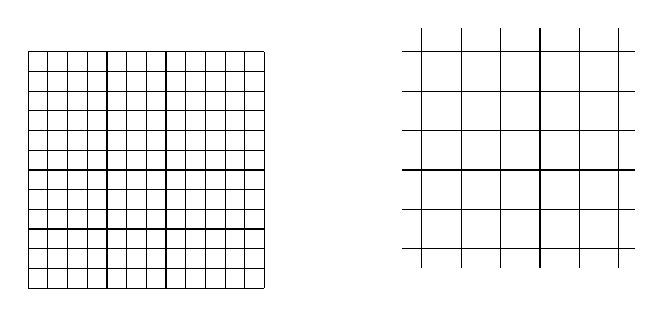
\begin{tikzpicture}
\draw[step=.25cm] (-1,-1) grid (2,2);
\draw[step=.5cm] (3.75,-.75) grid (6.7,2.3);
\end{tikzpicture}
%%%%%%%%%%%%%%%%%%%%%%%%%%%%%%%%% 
    \end{minipage}}} ;\node[fancytitle, right=10pt] at (box.north) {\hboxL{Output}};\node[fancytitle, left=-50pt] at (box.north west) {\hboxL{Input}};
\end{tikzpicture}\end{latin}
%____________________________________________



برای  رسم دایره و بیضی  مختصات مرکز و اندازه شعاع   به صورت زیر داده می‌شود. در خصوص بیضی شعاع بزرگ و کوچک داده می‌شود.
\begin{latin}
\begin{verbatim}
\draw(x,y) circle (r cm)
\ draw(x,y) ellipse (r_1cm  and  r_2cm)
\end{verbatim}
\end{latin}


%____________________________________________
 \begin{latin} \tikzstyle{mybox} = [draw=red, fill=gray!0, very thick,rectangle, inner sep=10pt, inner ysep=20pt]
\tikzstyle{fancytitle} =[fill=red, text=black]\begin{tikzpicture}
\node [mybox] (box){\begin{minipage}{0.42\textwidth}
\begin{footnotesize}\begin{verbatim}
 %******************************
\begin{tikzpicture}
\draw[line width=2pt] (0,0) circle (1cm);
\draw [line width=2pt](3,1) circle (.5cm);
\draw [line width=2pt](3,0) ellipse (1cm and .75cm);
\end{tikzpicture}
%*******************************
\end{verbatim}\end{footnotesize}
    \end{minipage}
\fboxrule=1mm\fbox{  \begin{minipage}{0.42\textwidth}
%%%%%%%%%%%%%%%%%%%%%%%%%%%%%%%%%%
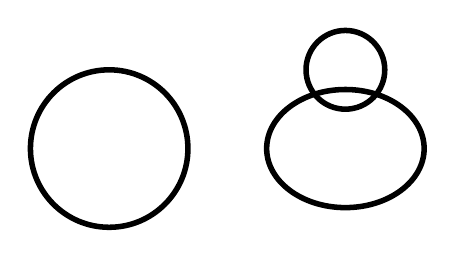
\begin{tikzpicture}
\draw[line width=2pt] (0,0) circle (1cm);
\draw [line width=2pt](3,1) circle (.5cm);
\draw [line width=2pt](3,0) ellipse (1cm and .75cm);
\end{tikzpicture}
%%%%%%%%%%%%%%%%%%%%%%%%%%%%%%%%% 
    \end{minipage}}} ;\node[fancytitle, right=10pt] at (box.north) {\hboxL{Output}};\node[fancytitle, left=-50pt] at (box.north west) {\hboxL{Input}};
\end{tikzpicture}\end{latin}
%____________________________________________


برای رنگ کردن داخل نواحی بسته هم می‌توان 
از دستورهای 
\lr{fill}
و
\lr{filldraw}
استفاده کرد و هم می‌توان 
\lr{fill}
را به صورت یک آپشن اختیاری استفاده کرد. دستور دیگر 
\lr{shade}
و 
\lr{shadedraw}
نیز وجود دارد که در مثال زیر خروجی آن را می‌بینید.

%_______________________________________________
 \begin{latin} \tikzstyle{mybox} = [draw=red, fill=gray!0, very thick,rectangle, inner sep=10pt, inner ysep=20pt]
\tikzstyle{fancytitle} =[fill=red, text=black]\begin{tikzpicture}
\node [mybox] (box){\begin{minipage}{0.42\textwidth}
\begin{footnotesize}\begin{verbatim}
 %******************************
\begin{tikzpicture}
\fill[green!20!white,ultra thick] (0,0) rectangle (1,1);
\draw [fill=red,ultra thick] (2,0) rectangle (3,1);
\filldraw [blue, fill=blue] 
(4,0) -- (5,1) -- (4.75,0.15) -- (4,0);
\draw [fill] (7,0.5) circle [radius=0.4];
\draw [fill=orange] (0,2) rectangle (2,3);
\draw [fill=white] (3,2) rectangle (5,3.5);
\shade[top color=yellow,bottom color=black]
 (0,-1) rectangle (2,-2);
\shadedraw[inner color=yellow,
outer color=red,draw=black] 
(3,-3) rectangle +(2,1);
\shade[left color=yellow,right color=black]
 (6,-2) rectangle +(1,1);
\shadedraw[inner color=yellow,
outer color=red,draw=yellow] (5,-3) rectangle +(2,1);
\shade[ball  color=yellow] (0,-2.50) circle (.5cm);
\end{tikzpicture}
%*******************************
\end{verbatim}\end{footnotesize}
    \end{minipage}
\fboxrule=1mm\fbox{  \begin{minipage}{0.42\textwidth}
%%%%%%%%%%%%%%%%%%%%%%%%%%%%%%%%%%
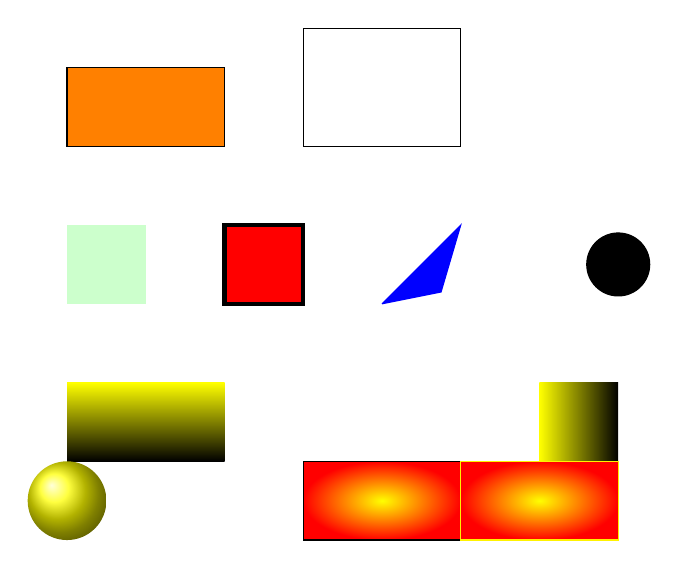
\begin{tikzpicture}
\fill[green!20!white,ultra thick] (0,0) rectangle (1,1);
\draw [fill=red,ultra thick] (2,0) rectangle (3,1);
\filldraw [blue, fill=blue] (4,0) -- (5,1) -- (4.75,0.15) -- (4,0);
\draw [fill] (7,0.5) circle [radius=0.4];
\draw [fill=orange] (0,2) rectangle (2,3);
\draw [fill=white] (3,2) rectangle (5,3.5);
\shade[top color=yellow,bottom color=black] (0,-1) rectangle (2,-2);
\shadedraw[inner color=yellow,outer color=red,draw=black] 
(3,-3) rectangle +(2,1);
\shade[left color=yellow,right color=black] (6,-2) rectangle +(1,1);
\shadedraw[inner color=yellow,outer color=red,draw=yellow] (5,-3) rectangle +(2,1);
\shade[ball  color=yellow] (0,-2.50) circle (.5cm);
\end{tikzpicture}
%%%%%%%%%%%%%%%%%%%%%%%%%%%%%%%%% 
    \end{minipage}}} ;\node[fancytitle, right=10pt] at (box.north) {\hboxL{Output}};\node[fancytitle, left=-50pt] at (box.north west) {\hboxL{Input}};
\end{tikzpicture}\end{latin}
%____________________________________________



 رسم کمان یا بخش  از یک  دایره‌ به مرکز $(x,y)$ و  شعاع $r$ را که از زاویه $\alpha$ شروع و به $beta$ ختم می‌شود. 
\begin{latin}\begin{verbatim}
\draw (x,y) arc (\alpha:\beta: r);$
\end{verbatim}\end{latin}
متذکر می‌شویم که
فرم قطبی یک نقطه به صورت $(\theta : r)$ می‌باشد. همچنین برای رسم کمانی از یک بیضی  کافیست در دستور بالا شعاع دوم بیضی نیز اضافه شود.\\
مثال:


%_______________________________________________
 \begin{latin} \tikzstyle{mybox} = [draw=red, fill=gray!0, very thick,rectangle, inner sep=10pt, inner ysep=20pt]
\tikzstyle{fancytitle} =[fill=red, text=black]\begin{tikzpicture}
\node [mybox] (box){\begin{minipage}{0.42\textwidth}
\begin{footnotesize}\begin{verbatim}
 %******************************
\begin{tikzpicture}
\draw (0,0) arc (10:80:1cm );
\draw (6,0) arc (0:250:1.75cm and 1cm);
\draw (0:1cm) -- (0:2cm)
arc (0:60:2cm) -- (60:1cm)
arc (60:0:1cm) -- cycle;
\end{tikzpicture}
%*******************************
\end{verbatim}\end{footnotesize}
    \end{minipage}
\fboxrule=1mm\fbox{  \begin{minipage}{0.42\textwidth}
%%%%%%%%%%%%%%%%%%%%%%%%%%%%%%%%%%
\begin{tikzpicture}
\draw (0,0) arc (10:80:1cm );
\draw (6,0) arc (0:250:1.75cm and 1cm);
\draw (0:1cm) -- (0:2cm)
arc (0:60:2cm) -- (60:1cm)
arc (60:0:1cm) -- cycle;
\end{tikzpicture}
%%%%%%%%%%%%%%%%%%%%%%%%%%%%%%%%% 
    \end{minipage}}} ;\node[fancytitle, right=10pt] at (box.north) {\hboxL{Output}};\node[fancytitle, left=-50pt] at (box.north west) {\hboxL{Input}};
\end{tikzpicture}\end{latin}
%____________________________________________


%_______________________________________________
 \begin{latin} \tikzstyle{mybox} = [draw=red, fill=gray!0, very thick,rectangle, inner sep=10pt, inner ysep=20pt]
\tikzstyle{fancytitle} =[fill=red, text=black]\begin{tikzpicture}
\node [mybox] (box){\begin{minipage}{0.42\textwidth}
\begin{footnotesize}\begin{verbatim}
 %******************************

\begin{tikzpicture}
\draw (0,0) -- (0:4) -- (30:3) -- cycle;
\filldraw[fill=blue!20!white, draw=black]
(0,0) -- (0:.5) arc (0:30:.5) -- cycle;
\end{tikzpicture}
%*******************************
\end{verbatim}\end{footnotesize}
    \end{minipage}
\fboxrule=1mm\fbox{  \begin{minipage}{0.42\textwidth}
%%%%%%%%%%%%%%%%%%%%%%%%%%%%%%%%%%

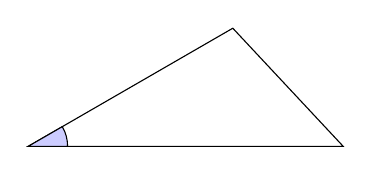
\begin{tikzpicture}
\draw (0,0) -- (0:4) -- (30:3) -- cycle;
\filldraw[fill=blue!20!white, draw=black]
(0,0) -- (0:.5) arc (0:30:.5) -- cycle;
\end{tikzpicture}
%%%%%%%%%%%%%%%%%%%%%%%%%%%%%%%%% 
    \end{minipage}}} ;\node[fancytitle, right=10pt,above=0pt] at (box.north) {\hboxL{Output}};\node[fancytitle, left=-50pt,above=0pt] at (box.north west) {\hboxL{Input}};
\end{tikzpicture}\end{latin}
%____________________________________________




%_______________________________________________
 \begin{latin} \tikzstyle{mybox} = [draw=red, fill=gray!0, very thick,rectangle, inner sep=10pt, inner ysep=20pt]
\tikzstyle{fancytitle} =[fill=red, text=black]\begin{tikzpicture}
\node [mybox] (box){\begin{minipage}{0.42\textwidth}
\begin{footnotesize}\begin{verbatim}
 %******************************
\begin{tikzpicture}
\filldraw[thick,fill=black!10] (0,0) circle (1.3cm);
\draw(0,0) -- (100:1.3);
\draw (1.35cm,8mm) node[above]
 {$100^\circ$};
\draw(0,0) -- (180:1.3);
\draw (-10mm,10mm) node[above] {$80^\circ$};
\draw(0,0) -- (260:1.3);
\draw (-13mm,-13mm) node[above] {$80^\circ$};
\draw(0,0) -- (320:1.3);
\draw (4mm,-18mm) node[above] {$60^\circ$};
\draw(0,0) -- (0:1.3);
\draw (16mm,-9mm) node[above] {$40^\circ$};
\end{tikzpicture}
%*******************************
\end{verbatim}\end{footnotesize}
    \end{minipage}
\fboxrule=1mm\fbox{  \begin{minipage}{0.42\textwidth}
%%%%%%%%%%%%%%%%%%%%%%%%%%%%%%%%%%

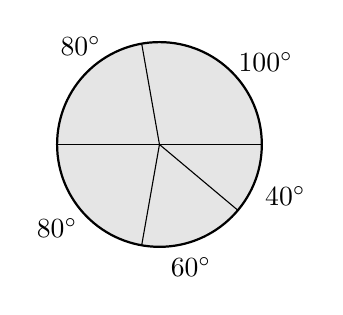
\begin{tikzpicture}
\filldraw[thick,fill=black!10] (0,0) circle (1.3cm);
\draw(0,0) -- (100:1.3);
\draw (1.35cm,8mm) node[above] {$100^\circ$};
\draw(0,0) -- (180:1.3);
\draw (-10mm,10mm) node[above] {$80^\circ$};
\draw(0,0) -- (260:1.3);\draw (-13mm,-13mm) node[above] {$80^\circ$};
\draw(0,0) -- (320:1.3);\draw (4mm,-18mm) node[above] {$60^\circ$};
\draw(0,0) -- (0:1.3);\draw (16mm,-9mm) node[above] {$40^\circ$};
\end{tikzpicture}
%%%%%%%%%%%%%%%%%%%%%%%%%%%%%%%%% 
    \end{minipage}}} ;\node[fancytitle, right=10pt,above=0pt] at (box.north) {\hboxL{Output}};\node[fancytitle, left=-50pt,above=0pt] at (box.north west) {\hboxL{Input}};
\end{tikzpicture}\end{latin}
%____________________________________________

%_______________________________________________
 \begin{latin} \tikzstyle{mybox} = [draw=red, fill=gray!0, very thick,rectangle, inner sep=10pt, inner ysep=20pt]
\tikzstyle{fancytitle} =[fill=red, text=black]\begin{tikzpicture}
\node [mybox] (box){\begin{minipage}{0.42\textwidth}
\begin{footnotesize}\begin{verbatim}
 %******************************
\begin{tikzpicture}
\filldraw[red!20!white]
 (0,0) -- (2,0) arc (0:50:2cm) -- (0,0);
\fill[green!60!white] 
 (0,0) -- (50:2) arc (50:180:2) -- (0,0);
\end{tikzpicture}
%*******************************
\end{verbatim}\end{footnotesize}
    \end{minipage}
\fboxrule=1mm\fbox{  \begin{minipage}{0.42\textwidth}
%%%%%%%%%%%%%%%%%%%%%%%%%%%%%%%%%%


\begin{tikzpicture}
\filldraw[red!20!white] (0,0) -- (2,0) arc (0:50:2cm) -- (0,0);
\fill[green!60!white]  (0,0) -- (50:2) arc (50:180:2) -- (0,0);
\end{tikzpicture}
%%%%%%%%%%%%%%%%%%%%%%%%%%%%%%%%% 
    \end{minipage}}} ;\node[fancytitle, right=10pt,above=0pt] at (box.north) {\hboxL{Output}};\node[fancytitle, left=-50pt,above=0pt] at (box.north west) {\hboxL{Input}};
\end{tikzpicture}\end{latin}
%____________________________________________


%_______________________________________________
 \begin{latin} \tikzstyle{mybox} = [draw=red, fill=gray!0, very thick,rectangle, inner sep=10pt, inner ysep=20pt]
\tikzstyle{fancytitle} =[fill=red, text=black]\begin{tikzpicture}
\node [mybox] (box){\begin{minipage}{0.42\textwidth}
\begin{footnotesize}\begin{verbatim}
 %******************************
\begin{tikzpicture}
\filldraw[fill=blue!20!white, 
draw=red!50!black,]
(0,0) -- (2,0) arc (0:30:2) -- (0,0);
\filldraw[fill=blue!20!white,
 draw=red!50!black]
(3,0) -- (5,0) arc (0:30:2) -- cycle;
\end{tikzpicture}
%*******************************
\end{verbatim}\end{footnotesize}
    \end{minipage}
\fboxrule=1mm\fbox{  \begin{minipage}{0.42\textwidth}
%%%%%%%%%%%%%%%%%%%%%%%%%%%%%%%%%%
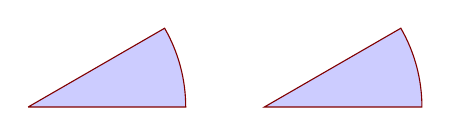
\begin{tikzpicture}
\filldraw[fill=blue!20!white, 
draw=red!50!black,]
(0,0) -- (2,0) arc (0:30:2) -- (0,0);
\filldraw[fill=blue!20!white, draw=red!50!black]
(3,0) -- (5,0) arc (0:30:2) -- cycle;
\end{tikzpicture}
%%%%%%%%%%%%%%%%%%%%%%%%%%%%%%%%% 
    \end{minipage}}} ;\node[fancytitle, right=10pt,above=0pt] at (box.north) {\hboxL{Output}};\node[fancytitle, left=-50pt,above=0pt] at (box.north west) {\hboxL{Input}};
\end{tikzpicture}\end{latin}


%____________________________________________


%_______________________________________________
 \begin{latin} \tikzstyle{mybox} = [draw=red, fill=gray!0, very thick,rectangle, inner sep=10pt, inner ysep=20pt]
\tikzstyle{fancytitle} =[fill=red, text=black]\begin{tikzpicture}
\node [mybox] (box){\begin{minipage}{0.42\textwidth}
\begin{footnotesize}\begin{verbatim}
 %******************************
\begin{tikzpicture}
\shadedraw[left color=red!90
,right color=green!80, draw=blue]
(0,0) -- (2,0) arc (0:60:2) -- cycle;
\end{tikzpicture}
%*******************************
\end{verbatim}\end{footnotesize}
    \end{minipage}
\fboxrule=1mm\fbox{  \begin{minipage}{0.42\textwidth}
%%%%%%%%%%%%%%%%%%%%%%%%%%%%%%%%%%
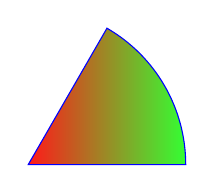
\begin{tikzpicture}
\shadedraw[left color=red!90,right color=green!80, draw=blue]
(0,0) -- (2,0) arc (0:60:2) -- cycle;
\end{tikzpicture}
%%%%%%%%%%%%%%%%%%%%%%%%%%%%%%%%% 
    \end{minipage}}} ;\node[fancytitle, right=10pt,above=0pt] at (box.north) {\hboxL{Output}};\node[fancytitle, left=-50pt,above=0pt] at (box.north west) {\hboxL{Input}};
\end{tikzpicture}\end{latin}
%____________________________________________


مثال
%_______________________________________________
 \begin{latin} \tikzstyle{mybox} = [draw=red, fill=gray!0, very thick,rectangle, inner sep=10pt, inner ysep=20pt]
\tikzstyle{fancytitle} =[fill=red, text=black]\begin{tikzpicture}
\node [mybox] (box){\begin{minipage}{0.42\textwidth}
\begin{footnotesize}\begin{verbatim}
 %******************************
\begin{tikzpicture}
\draw (0,0) -- (4,0) -- (3,2) -- cycle;
\filldraw[fill=blue!20!white, draw=black]
(0,0) -- (.5,0) arc (0:33:.5) -- cycle;
\filldraw[fill=blue!20!white, draw=black]
(4,0) -- (3.5,0) arc (180:117:.5) -- cycle;
\end{tikzpicture}
%*******************************
\end{verbatim}\end{footnotesize}
    \end{minipage}
\fboxrule=1mm\fbox{  \begin{minipage}{0.42\textwidth}
%%%%%%%%%%%%%%%%%%%%%%%%%%%%%%%%%%
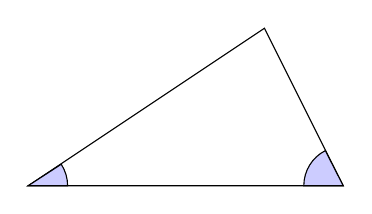
\begin{tikzpicture}
\draw (0,0) -- (4,0) -- (3,2) -- cycle;
\filldraw[fill=blue!20!white, draw=black]
(0,0) -- (.5,0) arc (0:33:.5) -- cycle;
\filldraw[fill=blue!20!white, draw=black]
(4,0) -- (3.5,0) arc (180:117:.5) -- cycle;
\end{tikzpicture}
%%%%%%%%%%%%%%%%%%%%%%%%%%%%%%%%% 
    \end{minipage}}} ;\node[fancytitle, right=10pt,above=0pt] at (box.north) {\hboxL{Output}};\node[fancytitle, left=-50pt,above=0pt] at (box.north west) {\hboxL{Input}};
\end{tikzpicture}\end{latin}
%____________________________________________

هنگامی که در رسم شکل از یک نقطه چند باز استفاده می‌شود یا  می‌خواهیم نام و برچسبی به نقطه‌ای خاص اختصاص دهیم بهتر است این نقطه را بصورت زیر ذخیره نماییم
\begin{latin}
\begin{verbatim}
\path (a,b) coordinate (name);
\path (angle: r) coordinate (name);
\coordinate (name)  at (a,b);
\coordinate (name) at (angle: r)
\end{verbatim}
\end{latin}

مثال 

%_______________________________________________
 \begin{latin} \tikzstyle{mybox} = [draw=red, fill=gray!0, very thick,rectangle, inner sep=10pt, inner ysep=20pt]
\tikzstyle{fancytitle} =[fill=red, text=black]\begin{tikzpicture}
\node [mybox] (box){\begin{minipage}{0.42\textwidth}
\begin{footnotesize}\begin{verbatim}
 %******************************
\begin{tikzpicture}
\path (0,0) coordinate (O);
\path (20: 3) coordinate (B);
\path (2, 2) coordinate (C);
\draw (O) -- (B) -- (C) -- cycle;
\end{tikzpicture}
%*******************************
\end{verbatim}\end{footnotesize}
    \end{minipage}
\fboxrule=1mm\fbox{  \begin{minipage}{0.42\textwidth}
%%%%%%%%%%%%%%%%%%%%%%%%%%%%%%%%%%
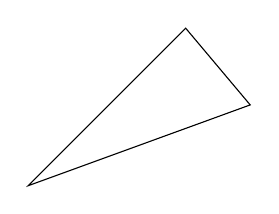
\begin{tikzpicture}
\path (0,0) coordinate (O);
\path (20: 3) coordinate (B);
\path (2, 2) coordinate (C);
\draw (O) -- (B) -- (C) -- cycle;
\end{tikzpicture}
%%%%%%%%%%%%%%%%%%%%%%%%%%%%%%%%% 
    \end{minipage}}} ;\node[fancytitle, right=10pt,above=0pt] at (box.north) {\hboxL{Output}};\node[fancytitle, left=-50pt,above=0pt] at (box.north west) {\hboxL{Input}};
\end{tikzpicture}\end{latin}
%_____

می‌توان مختصات یک نقطه را با اضافه کردن مقادیری دلخواه به مولفه‌های نقطه‌دیگری ذخیره نمود. برای نمونه در مثال زیر نقطه $B(2,1)$   با استفاده از نقطه $A(1,-1)$ به صورت 
$\ba path (A)\ ++(1,2) coordinate (B)$
 بدست آمده است
 %____________________________________________
 \begin{latin} \tikzstyle{mybox} = [draw=red, fill=gray!0, very thick,rectangle, inner sep=10pt, inner ysep=20pt]
\tikzstyle{fancytitle} =[fill=red, text=black]\begin{tikzpicture}
\node [mybox] (box){\begin{minipage}{0.42\textwidth}
\begin{footnotesize}\begin{verbatim}
 %******************************
\begin{tikzpicture}
\path (1,-1) coordinate (A);
\path (A) ++(1,2) coordinate (B);
\draw[line width=2pt] (A) -- (B);
\end{tikzpicture}
%*******************************
\end{verbatim}\end{footnotesize}
    \end{minipage}
\fboxrule=1mm\fbox{  \begin{minipage}{0.42\textwidth}
%%%%%%%%%%%%%%%%%%%%%%%%%%%%%%%%%%
\usetikzlibrary{arrows}

\begin{tikzpicture}
\path (1,-1) coordinate (A);
\path (A) ++(1,2) coordinate (B);
\draw[line width=2pt] (A) -- (B);
\end{tikzpicture}
%%%%%%%%%%%%%%%%%%%%%%%%%%%%%%%%% 
    \end{minipage}}} ;\node[fancytitle, right=10pt,above=0pt] at (box.north) {\hboxL{Output}};\node[fancytitle, left=-50pt,above=0pt] at (box.north west) {\hboxL{Input}};
\end{tikzpicture}\end{latin}
%____________________________________________
\ \\
مثال 
%____________________________________________
 \begin{latin} \tikzstyle{mybox} = [draw=red, fill=gray!0, very thick,rectangle, inner sep=10pt, inner ysep=20pt]
\tikzstyle{fancytitle} =[fill=red, text=black]\begin{tikzpicture}
\node [mybox] (box){\begin{minipage}{0.42\textwidth}
\begin{footnotesize}\begin{verbatim}
 %******************************
\begin{tikzpicture}[scale=1.2]
\coordinate  (A) at (0,0);
\coordinate  (B) at (1.5,.5);
\draw (A) -- (B);
\coordinate [label=left:$C$] (C) at (2,0);
\coordinate [label=right:$D$] (D) at (3.5,.5);
\draw (C) -- (D);
\end{tikzpicture}
%*******************************
\end{verbatim}\end{footnotesize}
    \end{minipage}
\fboxrule=1mm\fbox{  \begin{minipage}{0.42\textwidth}
%%%%%%%%%%%%%%%%%%%%%%%%%%%%%%%%%%
\begin{tikzpicture}[scale=1.2]
\coordinate  (A) at (0,0);
\coordinate  (B) at (1.5,.5);
\draw (A) -- (B);
\coordinate [label=left:$C$] (C) at (2,0);
\coordinate [label=right:$D$] (D) at (3.5,.5);
\draw (C) -- (D);
\end{tikzpicture}
%%%%%%%%%%%%%%%%%%%%%%%%%%%%%%%%% 
    \end{minipage}}} ;\node[fancytitle, right=10pt,above=0pt] at (box.north) {\hboxL{Output}};\node[fancytitle, left=-50pt,above=0pt] at (box.north west) {\hboxL{Input}};
\end{tikzpicture}\end{latin}
%____________________________________________
\ \\
گره‌ها را می‌توان با دستور 
\lr{node}
ایجاد کرد. دو مشخصه اصلی گره‌ها، فرم و متن آنها است. با استفاده گره‌ها می‌توان متون دلخواه را در دیاگرام‌ها وارد نمود. برای نمونه دستور  
\begin{latin}
\begin{verbatim}
\path (0,0) node[draw,shape=circle] (name) {$Circle$};
\end{verbatim}\end{latin}
یک گره به شکل دایره و مرکز مبدا مختصال به نام ‌ \lr{name} می‌سازد که متن آن \lr{Circle} است. آپشن \lr{draw} با عث می‌شود تا شکل تعیین شده (دراین مورد دایره ) رسم گردد. این حالت را می توان در مثال زیر مشاهده نمود.

مثال  \\
%____________________________________________
 \begin{latin} \tikzstyle{mybox} = [draw=red, fill=gray!0, very thick,rectangle]
\tikzstyle{fancytitle} =[fill=red, text=black]\begin{tikzpicture}
\node [mybox] (box){\begin{minipage}{0.42\textwidth}
\begin{footnotesize}\begin{verbatim}
 %******************************
\begin{tikzpicture}
\path (0,0) node[draw,shape=circle] (name) {$Circle$};
\path (2,0) node[shape=circle] (name) {$Circle$};
\path (4,0) node[draw
 ,shape=circle,inner sep=10pt] (name) {$Circle$};
\end{tikzpicture}
%*******************************
\end{verbatim}\end{footnotesize}
    \end{minipage}
\fboxrule=1mm\fbox{  \begin{minipage}{0.42\textwidth}
%%%%%%%%%%%%%%%%%%%%%%%%%%%%%%%%%%
\usetikzlibrary{arrows}
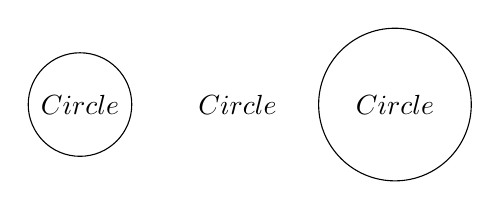
\begin{tikzpicture}
\path (0,0) node[draw,shape=circle] (name) {$Circle$};
\path (2,0) node[shape=circle] (name) {$Circle$};
\path (4,0) node[draw ,shape=circle,inner sep=10pt] (name) {$Circle$};
\end{tikzpicture}
%%%%%%%%%%%%%%%%%%%%%%%%%%%%%%%%% 
    \end{minipage}}} ;
    \node[fancytitle, left=-50pt,above=0pt] at (box.north) {\hboxL{Output}};\node[fancytitle, left=-50pt,above=0pt] at (box.north west) {\hboxL{Input}};
\end{tikzpicture}\end{latin}
%____________________________________________
\ \\
مثال 
\\
%____________________________________________
 \begin{latin} \tikzstyle{mybox} = [draw=red, fill=gray!0, very thick,rectangle]
\tikzstyle{fancytitle} =[fill=red, text=black]\begin{tikzpicture}
\node [mybox] (box){\begin{minipage}{0.42\textwidth}
\begin{footnotesize}\begin{verbatim}
 %******************************
\begin{tikzpicture} [xscale=.7]
 \tikzstyle{ann} = [fill=white,
 font=\footnotesize,inner sep=1pt]
\draw (0,0) -- (9,0);
\draw [>=latex, |<->|] 
(0,-0.5)--(3,-0.5);
\draw [>=open triangle 45
, <->] (3,-0.5)--(6,-0.5);
\draw [>=angle 60, |<->|] (6,-0.5)--(9,-0.5);
\draw (0,0) circle (2pt);
\node [above] at (0,0) {\lr{$x_1$}};
\draw (3,0) circle (2pt);
\node [above] at (3,0) {\lr{$x_0$}};
\draw (6,0) circle (2pt);
\node [above] at (6,0) {\lr{$x_2$}};
\draw (9,0) circle (2pt);
\node [above] at (9,0) {\lr{$x_3$}};
\node [ann] at (1.5,-0.5) {\lr{$ \frac{L}{3} $}};
\node [ann] at (4.5,-0.5) {\lr{$ \frac{L}{3} $}};
\node [ann] at (7.5,-0.5) {\lr{$ \frac{L}{3} $}};
\draw [>=triangle 90, |<->|] (0,-1)--(9,-1);
\node [ann] at (4.5,-1) {\lr{$ L$}};
%*******************************
\end{verbatim}\end{footnotesize}
    \end{minipage}
\fboxrule=1mm\fbox{  \begin{minipage}{0.42\textwidth}
%%%%%%%%%%%%%%%%%%%%%%%%%%%%%%%%%%
\begin{tikzpicture}[xscale=.7]
 \tikzstyle{ann} = [fill=white,font=\footnotesize,inner sep=1pt]
\draw (0,0) -- (9,0);
\draw [>=latex, |<->|] (0,-0.5)--(3,-0.5);
\draw [>=open triangle 45, <->] (3,-0.5)--(6,-0.5);
\draw [>=angle 60, |<->|] (6,-0.5)--(9,-0.5);
\draw (0,0) circle (2pt);
\node [above] at (0,0) {\lr{$x_1$}};
\draw (3,0) circle (2pt);
\node [above] at (3,0) {\lr{$x_0$}};
\draw (6,0) circle (2pt);
\node [above] at (6,0) {\lr{$x_2$}};
\draw (9,0) circle (2pt);
\node [above] at (9,0) {\lr{$x_3$}};
\node [ann] at (1.5,-0.5) {\lr{$ \frac{L}{3} $}};
\node [ann] at (4.5,-0.5) {\lr{$ \frac{L}{3} $}};
\node [ann] at (7.5,-0.5) {\lr{$ \frac{L}{3} $}};
\draw [>=triangle 90, |<->|] (0,-1)--(9,-1);
\node [ann] at (4.5,-1) {\lr{$ L$}};
\end{tikzpicture}
%%%%%%%%%%%%%%%%%%%%%%%%%%%%%%%%% 
    \end{minipage}}} ;
    \node[fancytitle, left=-50pt,above=0pt] at (box.north) {\hboxL{Output}};\node[fancytitle, left=-50pt,above=0pt] at (box.north west) {\hboxL{Input}};
\end{tikzpicture}\end{latin}
%____________________________________________




روش دیگر ایجاد گرده در نقطه‌ای به مختصات $(a,b)$ به صورت 
\begin{latin}
\begin{verbatim}
\node (name) at (a,b) {text};
\end{verbatim}\end{latin}
 می‌باشد. مثال قبل با این روش در زیر آورده شده است.

مثال  \\

%____________________________________________
 \begin{latin} \tikzstyle{mybox} = [draw=red, fill=gray!0, very thick,rectangle]
\tikzstyle{fancytitle} =[fill=red, text=black]\begin{tikzpicture}
\node [mybox] (box){\begin{minipage}{0.42\textwidth}
\begin{footnotesize}\begin{verbatim}
 %******************************
\begin{tikzpicture}
 \node [draw,shape=circle] (name) at (0,0)  {$Circle$};
\node [shape=circle]  (name) at (2,0) {$Circle$};
\end{tikzpicture}
%*******************************
\end{verbatim}\end{footnotesize}
    \end{minipage}
\fboxrule=1mm\fbox{  \begin{minipage}{0.42\textwidth}
%%%%%%%%%%%%%%%%%%%%%%%%%%%%%%%%%%
\usetikzlibrary{arrows}

\begin{tikzpicture}
\node [draw,shape=circle] (name) at (0,0)  {$Circle$};
\node [shape=circle]  (name) at (2,0) {$Circle$};
\end{tikzpicture}
%%%%%%%%%%%%%%%%%%%%%%%%%%%%%%%%% 
    \end{minipage}}} ;
    \node[fancytitle, left=-50pt,above=0pt] at (box.north) {\hboxL{Output}};\node[fancytitle, left=-50pt,above=0pt] at (box.north west) {\hboxL{Input}};
\end{tikzpicture}\end{latin}
%____________________________________________
چنانچه نقطه‌ای به مختصات  $(a,b)$ در یک ترسیم آورده شده باشد می‌توان با آوردن دستور \lr{node}   یک  گره در آن نقطه ایجاد نمود. با استفاده از آپشن‌هایی چون 
\begin{latin}

left,righ,above, below,east,west, ...
\end{latin}
 و یا ترکیب آین آپشن‌ها می‌توان محل الصاق برچسب با متن گره را مشخص نمود.
 
 مثال 
 \\
 
 %____________________________________________
 \begin{latin} \tikzstyle{mybox} = [draw=red, fill=gray!0, very thick,rectangle]
\tikzstyle{fancytitle} =[fill=red, text=black]\begin{tikzpicture}
\node [mybox] (box){\begin{minipage}{0.42\textwidth}
\begin{footnotesize}\begin{verbatim}

 %******************************
\begin{tikzpicture}
\draw [thick, <->] (0,2) -- (0,0) -- (2,0);
\draw[fill] (1,1) circle [radius=3mm];
\begin{scriptsize}
\node [below] at (1,1) {below};
\node [above] at (1,1) {above};
\node [left] at (1,1) {left};
\node [right] at (1,1) {right};
\end{scriptsize}
\end{tikzpicture}
%*******************************
\end{verbatim}\end{footnotesize}
    \end{minipage}
\fboxrule=1mm\fbox{  \begin{minipage}{0.42\textwidth}
%%%%%%%%%%%%%%%%%%%%%%%%%%%%%%%%%%
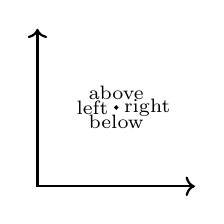
\begin{tikzpicture}
\draw [thick, <->] (0,2) -- (0,0) -- (2,0);
\draw[fill] (1,1) circle [radius=.2mm];
\begin{scriptsize}
\node [below] at (1,1) {below};
\node [above] at (1,1) {above};
\node [left] at (1,1) {left};
\node [right] at (1,1) {right};
\end{scriptsize}
\end{tikzpicture}
%%%%%%%%%%%%%%%%%%%%%%%%%%%%%%%%% 
    \end{minipage}}} ;
    \node[fancytitle, left=-50pt,above=0pt] at (box.north) {\hboxL{Output}};\node[fancytitle, left=-50pt,above=0pt] at (box.north west) {\hboxL{Input}};
\end{tikzpicture}\end{latin}
%____________________________________________


مثال 
 \\
 
 %____________________________________________
 \begin{latin} \tikzstyle{mybox} = [draw=red, fill=gray!0, very thick,rectangle]
\tikzstyle{fancytitle} =[fill=red, text=black]\begin{tikzpicture}
\node [mybox] (box){\begin{minipage}{0.42\textwidth}
\begin{footnotesize}\begin{verbatim}

 %******************************
\begin{tikzpicture}
\draw [thick, <->] (0,2) -- (0,0) -- (2,0);
\draw[fill] (1,1) circle [radius=.3mm];
\begin{scriptsize}
\node [below right] at (1,1) {below};
\node [above right] at (1,1) {above};
\node [below left] at (1,1) {left};
\node [above left] at (1,1) {right};
\end{scriptsize}
\end{tikzpicture}
%*******************************
\end{verbatim}\end{footnotesize}
    \end{minipage}
\fboxrule=1mm\fbox{  \begin{minipage}{0.42\textwidth}
%%%%%%%%%%%%%%%%%%%%%%%%%%%%%%%%%%
\begin{tikzpicture}
\draw [thick, <->] (0,2) -- (0,0) -- (2,0);
\draw[fill] (1,1) circle [radius=.2mm];
\begin{scriptsize}
\node [below right] at (1,1) {below};
\node [above right] at (1,1) {above};
\node [below left] at (1,1) {left};
\node [above left] at (1,1) {right};
\end{scriptsize}
\end{tikzpicture}
%%%%%%%%%%%%%%%%%%%%%%%%%%%%%%%%% 
    \end{minipage}}} ;
    \node[fancytitle, left=-50pt,above=0pt] at (box.north) {\hboxL{Output}};\node[fancytitle, left=-50pt,above=0pt] at (box.north west) {\hboxL{Input}};
\end{tikzpicture}\end{latin}
%____________________________________________


 
 مثال \\
 
 
%____________________________________________
 \begin{latin} \tikzstyle{mybox} = [draw=red, fill=gray!0, very thick,rectangle]
\tikzstyle{fancytitle} =[fill=red, text=black]\begin{tikzpicture}
\node [mybox] (box){\begin{minipage}{0.42\textwidth}
\begin{footnotesize}\begin{verbatim}

 %******************************
 \begin{tikzpicture}[xscale=1.5]
\draw [thick] (0,0) node
[below left]{$A$} -- (2,0) node
[below right]{$B$} -- (.5,1)
node[above]{$C$} --(0,0);
\end{tikzpicture}
%*******************************
\end{verbatim}\end{footnotesize}
    \end{minipage}
\fboxrule=1mm\fbox{  \begin{minipage}{0.42\textwidth}
%%%%%%%%%%%%%%%%%%%%%%%%%%%%%%%%%%
 \begin{tikzpicture}[xscale=1.5]
\draw [thick] (0,0) node
[below left]{$A$} -- (2,0) node[below right]{$B$} -- (.5,1)
node[above]{$C$} --(0,0);
\end{tikzpicture}
%%%%%%%%%%%%%%%%%%%%%%%%%%%%%%%%% 
    \end{minipage}}} ;
    \node[fancytitle, left=-50pt,above=0pt] at (box.north) {\hboxL{Output}};\node[fancytitle, left=-50pt,above=0pt] at (box.north west) {\hboxL{Input}};
\end{tikzpicture}\end{latin}
%____________________________________________

 
با استفاده از گره‌ها به راحتی می‌توان نمودارهایی مانند نمودار گرافها را رسم نمود. کافیست  مختصات رئوس گراف را به صورت گره ذخیره و با دستور رسم خط این گره‌ها را وصل نمود
\\
مثال



%____________________________________________
 \begin{latin} \tikzstyle{mybox} = [draw=red, fill=gray!0, very thick,rectangle]
\tikzstyle{fancytitle} =[fill=red, text=black]\begin{tikzpicture}
\node [mybox] (box){\begin{minipage}{0.42\textwidth}
\begin{footnotesize}\begin{verbatim}
 %******************************
\begin{tikzpicture}
\tikzstyle{every node}=[draw,shape=circle];
\path (0:0cm)
node (v0) {$v_0$};
\path (0:1cm)
node (v1) {$v_1$};
\path (72:1cm)
node (v2) {$v_2$};
\path (2*72:1cm) node (v3) {$v_3$};
\path (3*72:1cm) node (v4) {$v_4$};
\path (4*72:1cm) node (v5) {$v_5$};
\draw (v0) -- (v1)
(v0) -- (v2)
(v0) -- (v3)
(v0) -- (v4)
(v0) -- (v5);
\end{tikzpicture}
%*******************************
\end{verbatim}\end{footnotesize}
    \end{minipage}
\fboxrule=1mm\fbox{  \begin{minipage}{0.42\textwidth}
%%%%%%%%%%%%%%%%%%%%%%%%%%%%%%%%%%
\begin{tikzpicture}
\tikzstyle{every node}=[draw,shape=circle];
\path (0:0cm)
node (v0) {$v_0$};
\path (0:1cm)
node (v1) {$v_1$};
\path (72:1cm)
node (v2) {$v_2$};
\path (2*72:1cm) node (v3) {$v_3$};
\path (3*72:1cm) node (v4) {$v_4$};
\path (4*72:1cm) node (v5) {$v_5$};
\draw (v0) -- (v1)
(v0) -- (v2)
(v0) -- (v3)
(v0) -- (v4)
(v0) -- (v5);
\end{tikzpicture}
%%%%%%%%%%%%%%%%%%%%%%%%%%%%%%%%% 
    \end{minipage}}} ;\node[fancytitle, right=10pt,above=0pt] at (box.north) {\hboxL{Output}};\node[fancytitle, left=-50pt,above=0pt] at (box.north west) {\hboxL{Input}};
\end{tikzpicture}\end{latin}
%____________________________________________











%____________________________________________
 \begin{latin} \tikzstyle{mybox} = [draw=red, fill=gray!0, very thick,rectangle]
\tikzstyle{fancytitle} =[fill=red, text=black]\begin{tikzpicture}
\node [mybox] (box){\begin{minipage}{0.42\textwidth}
\begin{footnotesize}\begin{verbatim}
 %******************************
\begin{tikzpicture}[auto=left,
every node/.style={circle,fill=gray!20}]
  \node (n1) at (0,0) {1};
  \node (n2) at (2,0)  {4};
  \node (n3) at (2.62,1.9)  {2};
  \node (n4) at (1,3.08) {5};
  \node (n5) at (-0.62,1.9)  {3};
    \foreach \x/\y in {n1/n2,n2/n3,n3/n4,n4/n5,n5/n1}'
    \draw (\x) -- (\y);
\end{tikzpicture}
%*******************************
\end{verbatim}\end{footnotesize}
    \end{minipage}
\fboxrule=1mm\fbox{  \begin{minipage}{0.42\textwidth}
%%%%%%%%%%%%%%%%%%%%%%%%%%%%%%%%%%
\begin{tikzpicture}[auto=left,every node/.style={circle,fill=gray!20}]
  \node (n1) at (0,0) {1};
  \node (n2) at (2,0)  {4};
  \node (n3) at (2.62,1.9)  {2};
  \node (n4) at (1,3.08) {5};
  \node (n5) at (-0.62,1.9)  {3};
    \foreach \x/\y in {n1/n2,n2/n3,n3/n4,n4/n5,n5/n1}'
    \draw (\x) -- (\y);
\end{tikzpicture}
%%%%%%%%%%%%%%%%%%%%%%%%%%%%%%%%% 
    \end{minipage}}} ;\node[fancytitle, right=10pt] at (box.north) {\hboxL{Output}};\node[fancytitle, left=-50pt] at (box.north west) {\hboxL{Input}};
\end{tikzpicture}\end{latin}
%____________________________________________


%____________________________________________
 \begin{latin} \tikzstyle{mybox} = [draw=red, fill=gray!0, very thick,rectangle]
\tikzstyle{fancytitle} =[fill=red, text=black]\begin{tikzpicture}
\node [mybox] (box){\begin{minipage}{0.42\textwidth}
\begin{footnotesize}\begin{verbatim}
 %******************************
\begin{tikzpicture}
  [xscale=.6,auto=left,
  every node/.style={circle,fill=blue!20}]
  \node (n6) at (1,10) {6};
  \node (n4) at (4,8)  {4};
  \node (n5) at (8,9)  {5};
  \node (n1) at (11,8) {1};
  \node (n2) at (9,6)  {2};
  \node (n3) at (5,5)  {3};
  \foreach \x/\y in 
  {n6/n4,n4/n5,n5/n1,n1/n2,n2/n5,n2/n3,n3/n4}
    \draw (\x) -- (\y);
\draw(n6) [out=10 , in=130] to (n1);
\end{tikzpicture}
%*******************************
\end{verbatim}\end{footnotesize}
    \end{minipage}
\fboxrule=1mm\fbox{  \begin{minipage}{0.42\textwidth}
%%%%%%%%%%%%%%%%%%%%%%%%%%%%%%%%%%
\begin{tikzpicture}
[xscale=.6,auto=left,every node/.style={circle,fill=blue!20}]
  \node (n6) at (1,10) {6};
  \node (n4) at (4,8)  {4};
  \node (n5) at (8,9)  {5};
  \node (n1) at (11,8) {1};
  \node (n2) at (9,6)  {2};
  \node (n3) at (5,5)  {3};
  \foreach \x/\y in {n6/n4,n4/n5,n5/n1,n1/n2,n2/n5,n2/n3,n3/n4}
    \draw (\x) -- (\y);
\draw(n6) [out=10 , in=130] to (n1);
\end{tikzpicture}
%%%%%%%%%%%%%%%%%%%%%%%%%%%%%%%%% 
    \end{minipage}}} ;\node[fancytitle, right=10pt] at (box.north) {\hboxL{Output}};\node[fancytitle, left=-50pt] at (box.north west) {\hboxL{Input}};
\end{tikzpicture}\end{latin}
%____________________________________________

در دو مثال اخیر برای ترسیم یال‌ها از حلقه استفاده کردیم. فرم  حلقه به صورت 

\begin{latin}\begin{verbatim}
\foreach \var in {iteration list}
{
loop body
}\end{verbatim}
\end{latin}

مثال 

%____________________________________________
 \begin{latin} \tikzstyle{mybox} = [draw=red, fill=gray!0, very thick,rectangle]
\tikzstyle{fancytitle} =[fill=red, text=black]\begin{tikzpicture}
\node [mybox] (box){\begin{minipage}{0.42\textwidth}
\begin{footnotesize}\begin{verbatim}


 %******************************
\begin{tikzpicture}
  \foreach \x in {0,1,...,10}
    \draw (\x,1) -- (\x,1);
\end{tikzpicture}
%*******************************
\end{verbatim}\end{footnotesize}
    \end{minipage}
\fboxrule=1mm\fbox{  \begin{minipage}{0.42\textwidth}
%%%%%%%%%%%%%%%%%%%%%%%%%%%%%%%%%%
\begin{tikzpicture}
  \foreach \x in {0,1,2,3,4}
    \draw (\x,1) -- (1+\x,2);
\end{tikzpicture}
%%%%%%%%%%%%%%%%%%%%%%%%%%%%%%%%% 
    \end{minipage}}} ;\node[fancytitle, right=10pt] at (box.north) {\hboxL{Output}};\node[fancytitle, left=-50pt] at (box.north west) {\hboxL{Input}};
\end{tikzpicture}\end{latin}
%____________________________________________



%____________________________________________
 \begin{latin} \tikzstyle{mybox} = [draw=red, fill=gray!0, very thick,rectangle, inner sep=10pt, inner ysep=20pt]
\tikzstyle{fancytitle} =[fill=red, text=black]\begin{tikzpicture}
\node [mybox] (box){\begin{minipage}{0.42\textwidth}
\begin{footnotesize}\begin{verbatim}
 
 
 %******************************
\begin{tikzpicture}
\foreach \i in {1,...,4}
{
\path (\i,0) coordinate (X\i);
\fill (X\i) circle (6pt);
\draw (X\i) ++(0,-1) circle (6pt);
}
\end{tikzpicture}
%*******************************
\end{verbatim}\end{footnotesize}
    \end{minipage}
\fboxrule=1mm\fbox{  \begin{minipage}{0.42\textwidth}
%%%%%%%%%%%%%%%%%%%%%%%%%%%%%%%%%%
\begin{tikzpicture}\foreach \i in {1,...,4}
{
\path (\i,0) coordinate (X\i);
\fill (X\i) circle (6pt);
\draw (X\i) ++(0,-1) circle (6pt);
}\end{tikzpicture}
%%%%%%%%%%%%%%%%%%%%%%%%%%%%%%%%% 
    \end{minipage}}} ;\node[fancytitle, right=10pt] at (box.north) {\hboxL{Output}};\node[fancytitle, left=-50pt] at (box.north west) {\hboxL{Input}};
\end{tikzpicture}\end{latin}
%____________________________________________


بجای دادن مختصات برای تعریف گره 
می‌توان  مکان یک گره‌  را نسبت به گره دیگری مشخص نمود 
\\
   
   مثال



%____________________________________________
 \begin{latin} \tikzstyle{mybox} = [draw=red, fill=gray!0, very thick,rectangle]
\tikzstyle{fancytitle} =[fill=red, text=black]\begin{tikzpicture}
\node [mybox] (box){\begin{minipage}{0.42\textwidth}
\begin{footnotesize}\begin{verbatim}
  
 %******************************
\tikzset{node distance=2cm, auto}
\begin{tikzpicture}
  \node (C) {$C$};
  \node (P) [below of=C]
   {$\prod_{i \in I} A_i$};
  \node (Ai) [right of=P] {$A_i$};
  \draw[->] (C) to node {$f_i$} (Ai);
  \draw[->, dashed] (C) to node [swap] 
  {$\langle f_i \rangle_{i \in I}$} (P);
  \draw[->] (P) to node [swap] {$\pi_i$} (Ai);
\end{tikzpicture}
\end{tikzpicture}
%*******************************
\end{verbatim}\end{footnotesize}
    \end{minipage}
\fboxrule=1mm\fbox{  \begin{minipage}{0.42\textwidth}
%%%%%%%%%%%%%%%%%%%%%%%%%%%%%%%%%%
\tikzset{node distance=2cm, auto}
\begin{tikzpicture}
  \node (C) {$C$};
  \node (P) [below of=C] {$\prod_{i \in I} A_i$};
  \node (Ai) [right of=P] {$A_i$};
  \draw[->] (C) to node {$f_i$} (Ai);
  \draw[->, dashed] (C) to node [swap] {$\langle f_i \rangle_{i \in I}$} (P);
  \draw[->] (P) to node [swap] {$\pi_i$} (Ai);
\end{tikzpicture}
%%%%%%%%%%%%%%%%%%%%%%%%%%%%%%%%% 
    \end{minipage}}} ;\node[fancytitle, right=10pt] at (box.north) {\hboxL{Output}};\node[fancytitle, left=-50pt] at (box.north west) {\hboxL{Input}};
\end{tikzpicture}\end{latin}
%____________________________________________


مثال 

%____________________________________________
 \begin{latin} \tikzstyle{mybox} = [draw=red, fill=gray!0, very thick,rectangle]
\tikzstyle{fancytitle} =[fill=red, text=black]\begin{tikzpicture}
\node [mybox] (box){\begin{minipage}{0.42\textwidth}
\begin{footnotesize}\begin{verbatim}
  
 %******************************
\tikzset{node distance=2cm, auto}
\begin{tikzpicture}[line width=1.5pt]
  \node (P) {$P$};
  \node (B) [right of=P] {$B$};
  \node (A) [below of=P] {$A$};
  \node (C) [below of=B] {$C$};
  \node (P1) [node distance=1.94cm,
   left of=P, above of=P] {$\hat{P}$};
  \draw[->] (P) to node  {$\bar{f}$} (B);
  \draw[->] (P) to node [swap]
   {$\bar{g}$} (A);
  \draw[->] (A) to node [swap] {$f$} (C);
  \draw[->] (B) to node {$g$} (C);
  \draw[->, bend right ] (P1) 
  to node [swap] {$\hat{g}$} (A);
  \draw[->, bend left] (P1) to node
   {$\hat{f}$} (B);
  \draw[->, dashed] (P1) to node {$k$} (P);
\end{tikzpicture}
%*******************************
\end{verbatim}\end{footnotesize}
    \end{minipage}
\fboxrule=1mm\fbox{  \begin{minipage}{0.42\textwidth}
%%%%%%%%%%%%%%%%%%%%%%%%%%%%%%%%%%
\tikzset{node distance=2cm, auto}
\begin{tikzpicture}[line width=1.5pt]
  \node (P) {$P$};
  \node (B) [right of=P] {$B$};
  \node (A) [below of=P] {$A$};
  \node (C) [below of=B] {$C$};
  \node (P1) [node distance=1.94cm,
   left of=P, above of=P] {$\hat{P}$};
  \draw[->] (P) to node  {$\bar{f}$} (B);
  \draw[->] (P) to node [swap] {$\bar{g}$} (A);
  \draw[->] (A) to node [swap] {$f$} (C);
  \draw[->] (B) to node {$g$} (C);
  \draw[->, bend right ] (P1) 
  to node [swap] {$\hat{g}$} (A);
  \draw[->, bend left] (P1) to node 
  {$\hat{f}$} (B);
  \draw[->, dashed] (P1) to node {$k$} (P);
\end{tikzpicture}
%%%%%%%%%%%%%%%%%%%%%%%%%%%%%%%%% 
    \end{minipage}}} ;\node[fancytitle, right=10pt] at (box.north) {\hboxL{Output}};\node[fancytitle, left=-50pt] at (box.north west) {\hboxL{Input}};
\end{tikzpicture}\end{latin}
%____________________________________________

















 با استفاده از دستور 
 \lr{clip}
 می‌توان ناحیه ترسیم‌را محدود نمود. به عبارت دیگر این دستور  قسمت‌هایی از شکل که خارج از ناحیه مشخصی باشد را حذف می‌کند. 
 برای محدود کردن اثر 
 \lr{clip}
  از دستور 
 \lr{scope}
 استفاده می‌کنیم.
 برای نمونه دستور 
 \begin{latin}
 \begin{verbatim}
 \clip (0,0) circle (1cm) 
}\end{verbatim}
\end{latin}
 ناحیه ترسیم را محدود به دایره‌ای به شعاع ۱ سانتی‌متر و مبدا مختصات می‌کند. پس هر بخش از شکل که خارج این دایره باشد حذف می‌گردد. 
 
 مثال \\


%____________________________________________
 \begin{latin} \tikzstyle{mybox} = [draw=red, fill=gray!0, very thick,rectangle, inner sep=10pt, inner ysep=20pt]
\tikzstyle{fancytitle} =[fill=red, text=black]\begin{tikzpicture}
\node [mybox] (box){\begin{minipage}{0.42\textwidth}
\begin{footnotesize}\begin{verbatim}
  
 %******************************
\begin{tikzpicture}
\draw [fill=orange] (0,-1) rectangle (1,1);
\clip (2,.5) circle (1cm) ;
\draw [fill=orange] (2,-1) rectangle (3,0)
\end{tikzpicture}
%*******************************
\end{verbatim}\end{footnotesize}
    \end{minipage}
\fboxrule=1mm\fbox{  \begin{minipage}{0.42\textwidth}
%%%%%%%%%%%%%%%%%%%%%%%%%%%%%%%%%%
\begin{tikzpicture}
\draw [fill=orange] (0,-1) rectangle (1,1);
\clip (2,.5) circle (1cm) ;
\draw [fill=orange] (2,-1) rectangle (3,0);
\end{tikzpicture}
%%%%%%%%%%%%%%%%%%%%%%%%%%%%%%%%% 
   \end{minipage}}} ;\node[fancytitle, right=10pt] at (box.north) {\hboxL{Output}};\node[fancytitle, left=-50pt] at (box.north west) {\hboxL{Input}};
\end{tikzpicture}\end{latin}
%____________________________________________
\ \\
مثال 
%____________________________________________
 \begin{latin} \tikzstyle{mybox} = [draw=red, fill=gray!0, very thick,rectangle, inner sep=10pt, inner ysep=20pt]
\tikzstyle{fancytitle} =[fill=red, text=black]\begin{tikzpicture}
\node [mybox] (box){\begin{minipage}{0.42\textwidth}
\begin{footnotesize}\begin{verbatim}
  
 %******************************
\begin{tikzpicture}
\draw (0,0) circle (1cm) ;
\clip(0,0) circle (1cm) ;
\draw [fill=red] (1,0) circle (1cm) ;
\end{tikzpicture}
%*******************************
\end{verbatim}\end{footnotesize}
    \end{minipage}
\fboxrule=1mm\fbox{  \begin{minipage}{0.42\textwidth}
%%%%%%%%%%%%%%%%%%%%%%%%%%%%%%%%%%
\begin{tikzpicture}
\draw (0,0) circle (1cm) ;
\draw  (1,0) circle (1cm) ;
\clip(0,0) circle (1cm) ;
\draw [fill=red] (1,0) circle (1cm) ;
\end{tikzpicture}
%%%%%%%%%%%%%%%%%%%%%%%%%%%%%%%%% 
    \end{minipage}}} ;\node[fancytitle, right=10pt] at (box.north) {\hboxL{Output}};\node[fancytitle, left=-50pt] at (box.north west) {\hboxL{Input}};
\end{tikzpicture}\end{latin}
%____________________________________________

مثال با استفاده \lr{scope}

 %____________________________________________
 \begin{latin} \tikzstyle{mybox} = [draw=red, fill=gray!0, very thick,rectangle, inner sep=10pt, inner ysep=20pt]
\tikzstyle{fancytitle} =[fill=red, text=black]\begin{tikzpicture}
\node [mybox] (box){\begin{minipage}{0.42\textwidth}
\begin{footnotesize}\begin{verbatim}
  
 %******************************
\begin{tikzpicture}
\draw (-2, 1.5) rectangle (2, -1.5);
\begin{scope}
\clip (-0.5, 0) circle (1);
\clip ( 0.5, 0) circle (1);
\fill[color=gray] (-2,1.5)
rectangle (2,-1.5);
\end{scope}
\draw (-0.5, 0) circle (1);
\draw ( 0.5, 0) circle (1);
\end{tikzpicture}
%*******************************
\end{verbatim}\end{footnotesize}
    \end{minipage}
\fboxrule=1mm\fbox{  \begin{minipage}{0.42\textwidth}
%%%%%%%%%%%%%%%%%%%%%%%%%%%%%%%%%%
\begin{tikzpicture}
\draw (-2, 1.5) rectangle (2, -1.5);
\begin{scope}
\clip (-0.5, 0) circle (1);
\clip ( 0.5, 0) circle (1);
\fill[color=gray] (-2,1.5)
rectangle (2,-1.5);
\end{scope}
\draw (-0.5, 0) circle (1);
\draw ( 0.5, 0) circle (1);
\end{tikzpicture}
%%%%%%%%%%%%%%%%%%%%%%%%%%%%%%%%% 
    \end{minipage}}} ;\node[fancytitle, right=10pt] at (box.north) {\hboxL{Output}};\node[fancytitle, left=-50pt] at (box.north west) {\hboxL{Input}};
\end{tikzpicture}\end{latin}
%____________________________________________








\end{document}
